\documentclass[11pt]{article}

% Packages
\usepackage[utf8]{inputenc}
\usepackage{amsmath,amssymb,amsthm}
\usepackage{graphicx}
\usepackage[margin=1in]{geometry}
\usepackage{natbib}
\usepackage{hyperref}
\usepackage{xcolor}
\usepackage{float}
\usepackage{caption}
\usepackage{subcaption}

% Custom commands
\newcommand{\doi}[1]{\href{https://doi.org/#1}{doi:#1}}

% Title
\title{\textbf{Emergence of Tri-trophic Coexistence through Metabolic Niche Partitioning:\\
A Bifurcation Analysis of Cross-Feeding Microbial Communities}}

\author{Jian Wang\\
\small Department of Mathematics and Biology\\
\small [Institution]\\
\small \texttt{email@institution.edu}}

\date{\today}

\begin{document}

\maketitle

\begin{abstract}
Microbial communities often exhibit complex cross-feeding interactions where metabolic by-products of one species become resources for another. Understanding how generalist species can coexist with specialists in such communities remains a fundamental challenge in microbial ecology. Here, we develop a mathematical framework to analyze a three-species cross-feeding system consisting of two specialists (substrate and metabolite specialists) and one generalist capable of utilizing both pathways. Using dynamical systems theory and bifurcation analysis, we derive analytical conditions for species coexistence and identify critical transitions as the generalist shifts its metabolic strategy. We show that the generalist can invade the stable two-species consortium only within a specific parameter window, determined by the balance between its dual metabolic pathways. Our analysis reveals a transcritical bifurcation where increasing reliance on the substrate pathway enables generalist invasion, while excessive specialization leads to competitive exclusion of the metabolite specialist. These findings provide quantitative predictions for engineering stable synthetic microbial consortia and understanding metabolic diversity in natural communities.
\end{abstract}

\section{Introduction}

Microorganisms rarely live in isolation; instead, they form complex communities where species interact through the exchange of metabolic products \cite{goldford2018emergent,pacheco2019costless}. Cross-feeding interactions—where metabolic by-products of one species serve as resources for another—are ubiquitous in natural and engineered microbial systems \cite{ponomarova2017metabolic}. These syntrophic relationships can stabilize community structure, enhance productivity, and enable coexistence of species that would otherwise compete \cite{gore2009snowdrift,harcombe2014metabolic}.

A key question in microbial ecology is: how can generalist species, capable of utilizing multiple metabolic pathways, coexist with specialists in cross-feeding communities? This question is particularly relevant for understanding metabolic diversity and for rational design of synthetic consortia \cite{klitgord2010environments,zelezniak2015metabolic}. While pairwise interactions have been extensively studied both theoretically and experimentally \cite{momeni2011spatial,muller2014venn}, the dynamics of systems with both specialists and generalists remain poorly understood.

Here, we develop a rigorous mathematical framework to analyze a three-species cross-feeding model. Our system consists of: (i) a \textit{substrate specialist} (S) that produces metabolites, (ii) a \textit{metabolite specialist} (M) that obligately depends on S's by-products, and (iii) a \textit{generalist} (G) that can utilize both substrate and metabolite pathways. The generalist's metabolic strategy is controlled by a parameter $\omega \in [0,1]$ representing the relative investment in each pathway.

Using tools from dynamical systems theory, we systematically analyze: (1) pairwise interactions between all species pairs, (2) conditions for the generalist to invade the stable S-M consortium, and (3) the complete bifurcation structure as $\omega$ varies. Our analysis yields explicit analytical formulas for equilibrium points, stability criteria, and critical thresholds. We identify a transcritical bifurcation mechanism underlying the transition from two-species to three-species coexistence, providing quantitative predictions testable in experimental systems.

\section{Model Framework}

\subsection{Model Formulation}

We consider a well-mixed microbial community where population densities (scaled by carrying capacities) are denoted $s$, $m$, and $g$ for substrate specialist, metabolite specialist, and generalist, respectively. The dynamics are governed by:

\begin{align}
\frac{ds}{dt} &= r_S \cdot s \left(1 + \sigma_{SM} \cdot m + a \cdot g - s\right) \label{eq:s_dynamics}\\
\frac{dm}{dt} &= r_M \cdot m \left(-1 + \sigma_{MS} \cdot s + b \cdot g - m\right) \label{eq:m_dynamics}\\
\frac{dg}{dt} &= r_G \cdot g \left(d + c \cdot s + e \cdot m - g\right) \label{eq:g_dynamics}
\end{align}

where $r_S$, $r_M$, $r_G$ are intrinsic growth rates. The parameters represent net interactions:

\begin{itemize}
\item $\sigma_{SM}$: benefit to S from M's metabolites (cooperative)
\item $\sigma_{MS}$: benefit to M from S's by-products (obligate: $\sigma_{MS} > 1$ required for M survival)
\item $a = (1-\omega)\sigma_{SG} - \omega\alpha_{SG}$: net effect of G on S
\item $c = (1-\omega)\sigma_{GS} - \omega\alpha_{GS}$: net effect of S on G
\item $b = \omega\sigma_{MG} - (1-\omega)\alpha_{MG}$: net effect of G on M
\item $e = \omega\sigma_{GM} - (1-\omega)\alpha_{GM}$: net effect of M on G
\item $d = 2\omega - 1$: generalist's basal growth rate
\end{itemize}

The parameter $\omega \in [0,1]$ controls the generalist's metabolic strategy:
\begin{itemize}
\item $\omega = 0$: pure metabolite pathway (G behaves like M)
\item $\omega = 0.5$: balanced generalist
\item $\omega = 1$: pure substrate pathway (G behaves like S)
\end{itemize}

Crucially, all net interaction parameters $(a, b, c, d, e)$ are \textit{linear functions} of $\omega$, enabling analytical tractability.

\subsection{Biological Interpretation}

This model captures essential features of cross-feeding communities:

\textbf{Obligate mutualism (S-M):} M has negative basal growth ($-1$) and requires S's cross-feeding ($\sigma_{MS} > 1$) to survive. This represents strict metabolic dependence, as seen in syntrophic bacteria \cite{schink2002syntrophic}.

\textbf{Generalist flexibility:} The parameter $\omega$ represents evolutionary or physiological trade-offs in pathway usage. Low $\omega$ favors metabolite utilization (cooperation with M), while high $\omega$ favors substrate usage (competition with S).

\textbf{Net interactions:} Parameters $a$, $b$, $c$, $e$ combine cooperative ($\sigma$) and competitive ($\alpha$) effects, weighted by $\omega$. This captures the dual nature of generalist interactions: facilitating through one pathway while competing through another.

\section{Results}

\subsection{Section 1: Pairwise Interactions}

We first analyze all three pairwise subsystems to establish baseline dynamics.

\subsubsection{1.1 S-M System}

Setting $g = 0$ in Eqs.~\ref{eq:s_dynamics}-\ref{eq:m_dynamics}:

\begin{align}
\frac{ds}{dt} &= r_S \cdot s(1 + \sigma_{SM} \cdot m - s)\\
\frac{dm}{dt} &= r_M \cdot m(-1 + \sigma_{MS} \cdot s - m)
\end{align}

\textbf{Equilibrium Points:}

\begin{align}
E_1 &= (0, 0) \quad \text{(extinction)}\\
E_2 &= (1, 0) \quad \text{(S-only)}\\
E_3 &= \left(\frac{1-\sigma_{SM}}{1-\sigma_{SM}\cdot\sigma_{MS}}, \frac{\sigma_{MS}-1}{1-\sigma_{SM}\cdot\sigma_{MS}}\right) \quad \text{(coexistence)}
\end{align}

\textbf{Stability Analysis:}

The Jacobian at $E_3$ is:
\begin{equation}
J = \begin{pmatrix}
-r_S s^* & r_S s^* \sigma_{SM}\\
r_M m^* \sigma_{MS} & -r_M m^*
\end{pmatrix}
\end{equation}

Stability requires:
\begin{align}
\text{Tr}(J) &= -(r_S s^* + r_M m^*) < 0 \quad \checkmark \text{ (always satisfied)}\\
\det(J) &= r_S r_M s^* m^* (1 - \sigma_{SM}\cdot\sigma_{MS}) > 0
\end{align}

\textbf{Coexistence Condition:}
\begin{equation}
\boxed{\sigma_{MS} > 1 \quad \text{AND} \quad \sigma_{SM}\cdot\sigma_{MS} < 1}
\end{equation}

This states that M must receive sufficient benefit to overcome its negative basal rate ($\sigma_{MS} > 1$), but mutualism cannot be too strong or the system becomes unstable ($\sigma_{SM}\cdot\sigma_{MS} < 1$).

\subsubsection{1.2 S-G System}

Setting $m = 0$:

\begin{align}
\frac{ds}{dt} &= r_S \cdot s(1 + a \cdot g - s)\\
\frac{dg}{dt} &= r_G \cdot g(d + c \cdot s - g)
\end{align}

\textbf{Equilibrium Points:}

\begin{align}
E_1 &= (0, 0)\\
E_2 &= (1, 0) \quad \text{(S-only)}\\
E_3 &= (0, d) \quad \text{(G-only, if } d > 0 \text{)}\\
E_4 &= \left(\frac{1+ad}{1-ac}, \frac{d+c}{1-ac}\right) \quad \text{(coexistence)}
\end{align}

The coexistence equilibrium exists when $(d+c)$ and $(1-ac)$ have the same sign. Stability depends on the net interaction strengths.

\textbf{Key Observation:} G can survive alone ($E_3$) only when $\omega > 0.5$ (i.e., $d > 0$), reflecting its ability to use the substrate pathway independently.

\subsubsection{1.3 M-G System}

Setting $s = 0$:

\begin{align}
\frac{dm}{dt} &= r_M \cdot m(-1 + bg - m)\\
\frac{dg}{dt} &= r_G \cdot g(d + em - g)
\end{align}

\textbf{Equilibrium Points:}

\begin{align}
E_1 &= (0, 0)\\
E_2 &= (0, d) \quad \text{(G-only, if } d > 0 \text{)}\\
E_3 &= \left(\frac{bd-1}{1-be}, \frac{d+e}{1-be}\right) \quad \text{(coexistence)}
\end{align}

\textbf{Critical Insight:} M-G coexistence requires M to receive sufficient benefit from G ($b \cdot g^* > 1$). However, without S providing baseline resources, this is typically not feasible with our parameter regime.

\textbf{Summary Figure 1:} Phase portraits for all three pairwise systems show nullclines, equilibria (stable: filled circles; unstable: open circles), and representative trajectories. See Figure \ref{fig:pairwise}.

\begin{figure}[H]
\centering
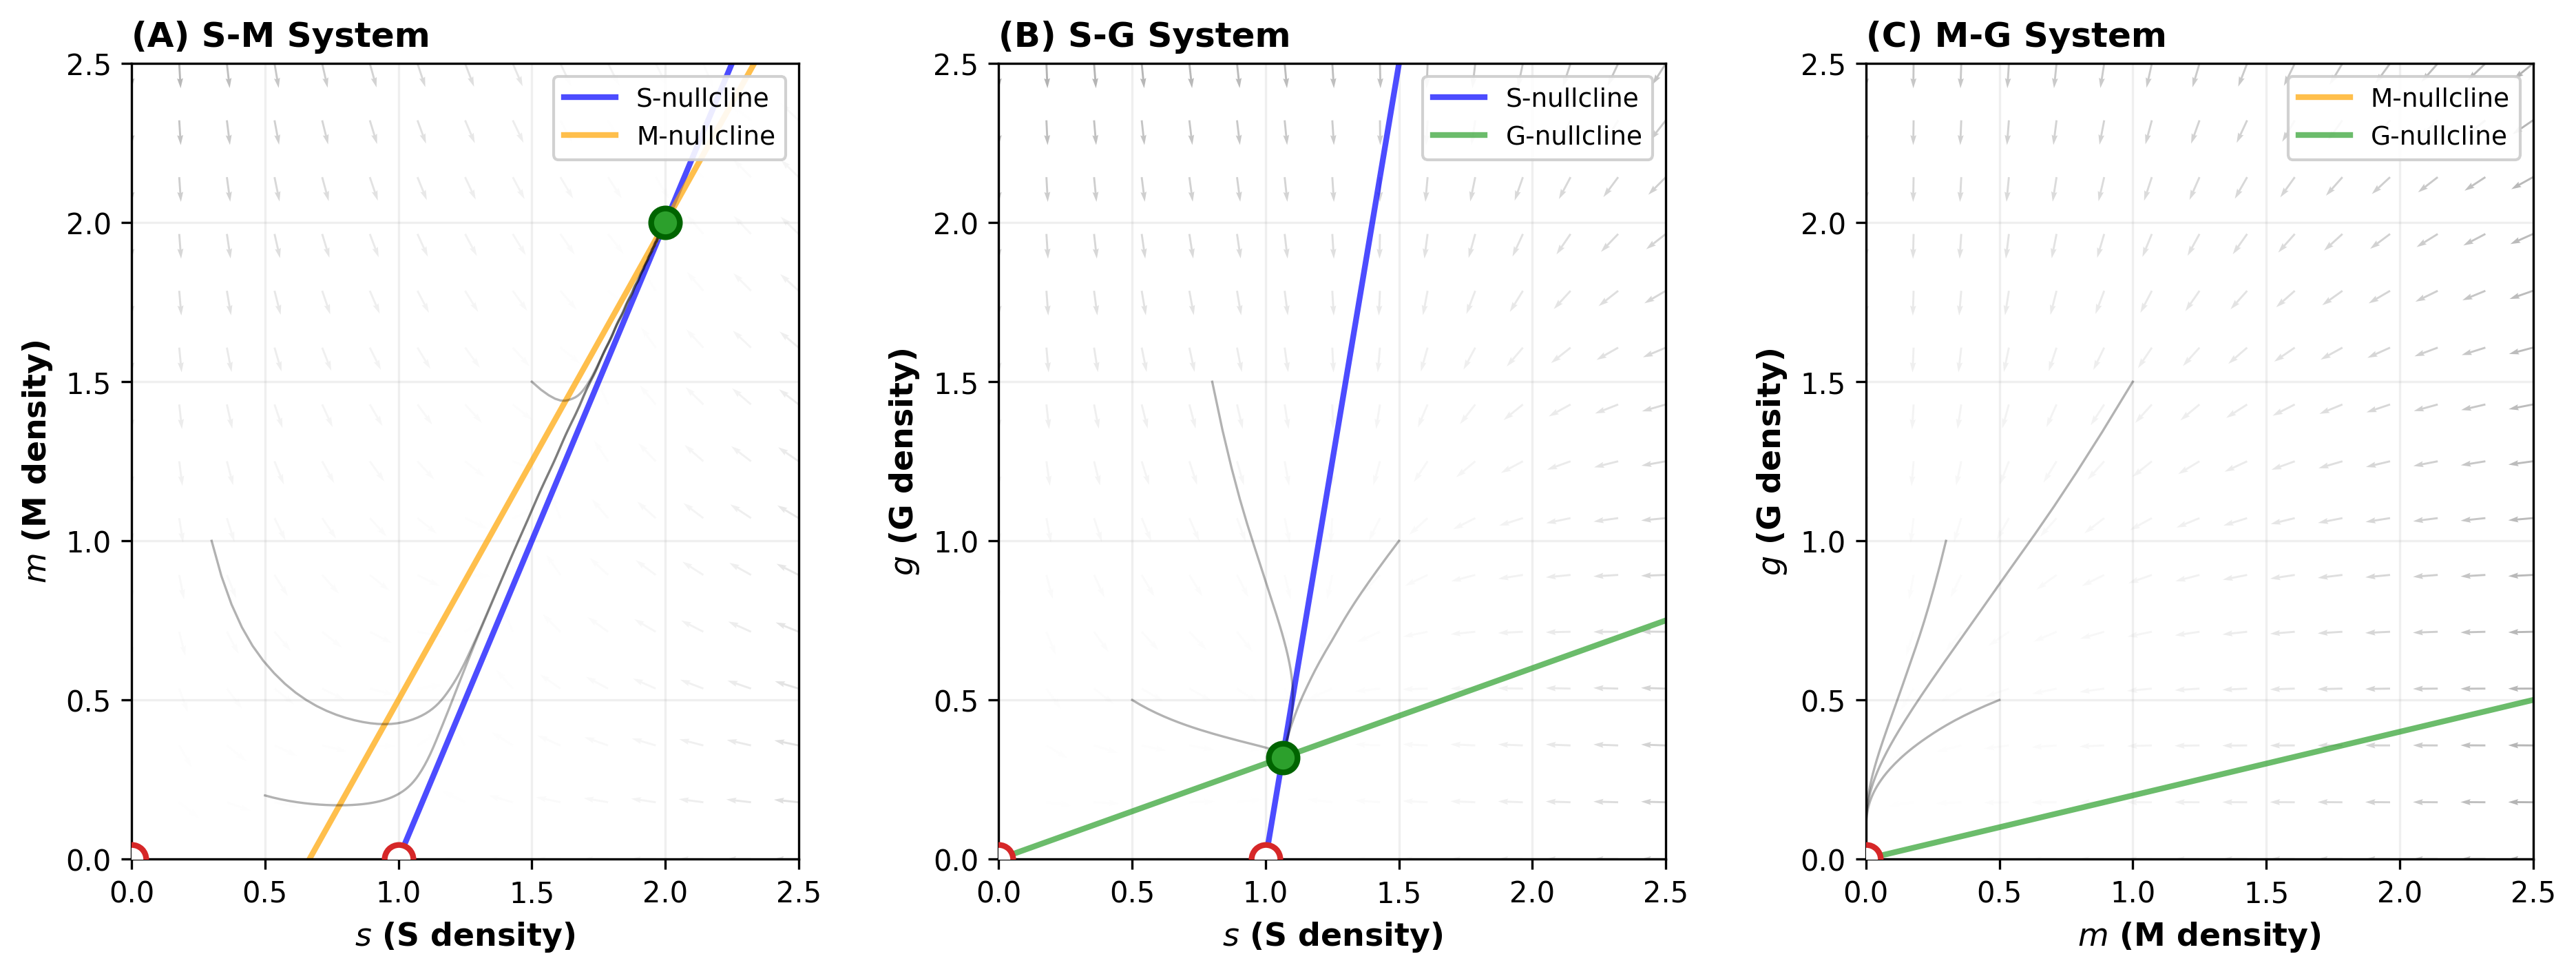
\includegraphics[width=\textwidth]{figures/Figure1_pairwise_systems.png}
\caption{\textbf{Pairwise interaction dynamics.} Phase portraits showing nullclines (colored lines), vector fields (gray arrows), equilibria (circles: filled = stable, open = unstable), and sample trajectories (black curves). (A) S-M system exhibits stable mutualistic coexistence when $\sigma_{MS} > 1$ and $\sigma_{MS}\cdot\sigma_{SM} < 1$. (B) S-G system shows coexistence dependent on $\omega$-controlled net interactions. (C) M-G system has limited coexistence due to M's obligate dependence.}
\label{fig:pairwise}
\end{figure}

\subsection{Section 2: Three-Species Dynamics}

\subsubsection{2.1 Equilibrium Structure}

The complete three-species system admits multiple equilibria:

\textbf{Boundary Equilibria:}
\begin{itemize}
\item $E_0 = (0, 0, 0)$: complete extinction
\item $E_S = (1, 0, 0)$: S-only
\item $E_{SM} = (s^*_{SM}, m^*_{SM}, 0)$: S-M coexistence (from Section 1.1)
\item $E_{SG} = (s^*_{SG}, 0, g^*_{SG})$: S-G coexistence (from Section 1.2)
\end{itemize}

\textbf{Interior Equilibrium:}
$E^* = (s^*, m^*, g^*)$ represents full three-species coexistence. This equilibrium satisfies:

\begin{align}
1 + \sigma_{SM} \cdot m^* + a \cdot g^* - s^* &= 0\\
-1 + \sigma_{MS} \cdot s^* + b \cdot g^* - m^* &= 0\\
d + c \cdot s^* + e \cdot m^* - g^* &= 0
\end{align}

This is a linear 3$\times$3 system that can be solved analytically (though expressions are lengthy) or numerically.

\subsubsection{2.2 Generalist Invasion of S-M Consortia}

A central question is: when can G invade the stable S-M equilibrium?

At $E_{SM} = (s^*_{SM}, m^*_{SM}, 0)$, the invasion fitness of G (rare species growth rate) is:

\begin{equation}
\lambda_G = r_G \left(d + c \cdot s^*_{SM} + e \cdot m^*_{SM}\right)
\end{equation}

where:
\begin{align}
s^*_{SM} &= \frac{1-\sigma_{SM}}{1-\sigma_{MS}\cdot\sigma_{SM}}\\
m^*_{SM} &= \frac{\sigma_{MS}-1}{1-\sigma_{MS}\cdot\sigma_{SM}}
\end{align}

\textbf{Invasion Criterion:}
\begin{equation}
\boxed{\text{G invades} \quad \Leftrightarrow \quad d + c \cdot s^*_{SM} + e \cdot m^*_{SM} > 0}
\end{equation}

Since $d$, $c$, $e$ are linear in $\omega$, this yields a \textit{critical value} $\omega_{crit}$:

\begin{equation}
\omega_{crit} = \frac{1 - \sigma_{GS} \cdot s^*_{SM} + \alpha_{GM} \cdot m^*_{SM}}{2 - (\sigma_{GS}+\alpha_{GS}) \cdot s^*_{SM} + (\sigma_{GM}+\alpha_{GM}) \cdot m^*_{SM}}
\end{equation}

For $\omega > \omega_{crit}$, the generalist successfully invades, triggering a transition from two-species to three-species community.

\textbf{Biological Interpretation:}
\begin{itemize}
\item At low $\omega$ (metabolite specialist), G competes strongly with M, reducing invasion fitness.
\item At intermediate $\omega$, G balances substrate and metabolite usage, enabling coexistence through niche partitioning.
\item The critical $\omega_{crit}$ depends on the S-M equilibrium densities, linking pairwise and trio dynamics.
\end{itemize}

Figure \ref{fig:invasion} panels A-B show $\lambda_G(\omega)$ and its components $(d, c \cdot s^*_{SM}, e \cdot m^*_{SM})$. The invasion rate crosses zero at $\omega_{crit}$, defining the bifurcation point. Panel C maps the invasion region in $(\omega, \sigma_{MS})$ parameter space, revealing a triangular coexistence zone. Panel D shows time series where G invades and establishes at $\omega = 0.6 > \omega_{crit}$.

\begin{figure}[H]
\centering
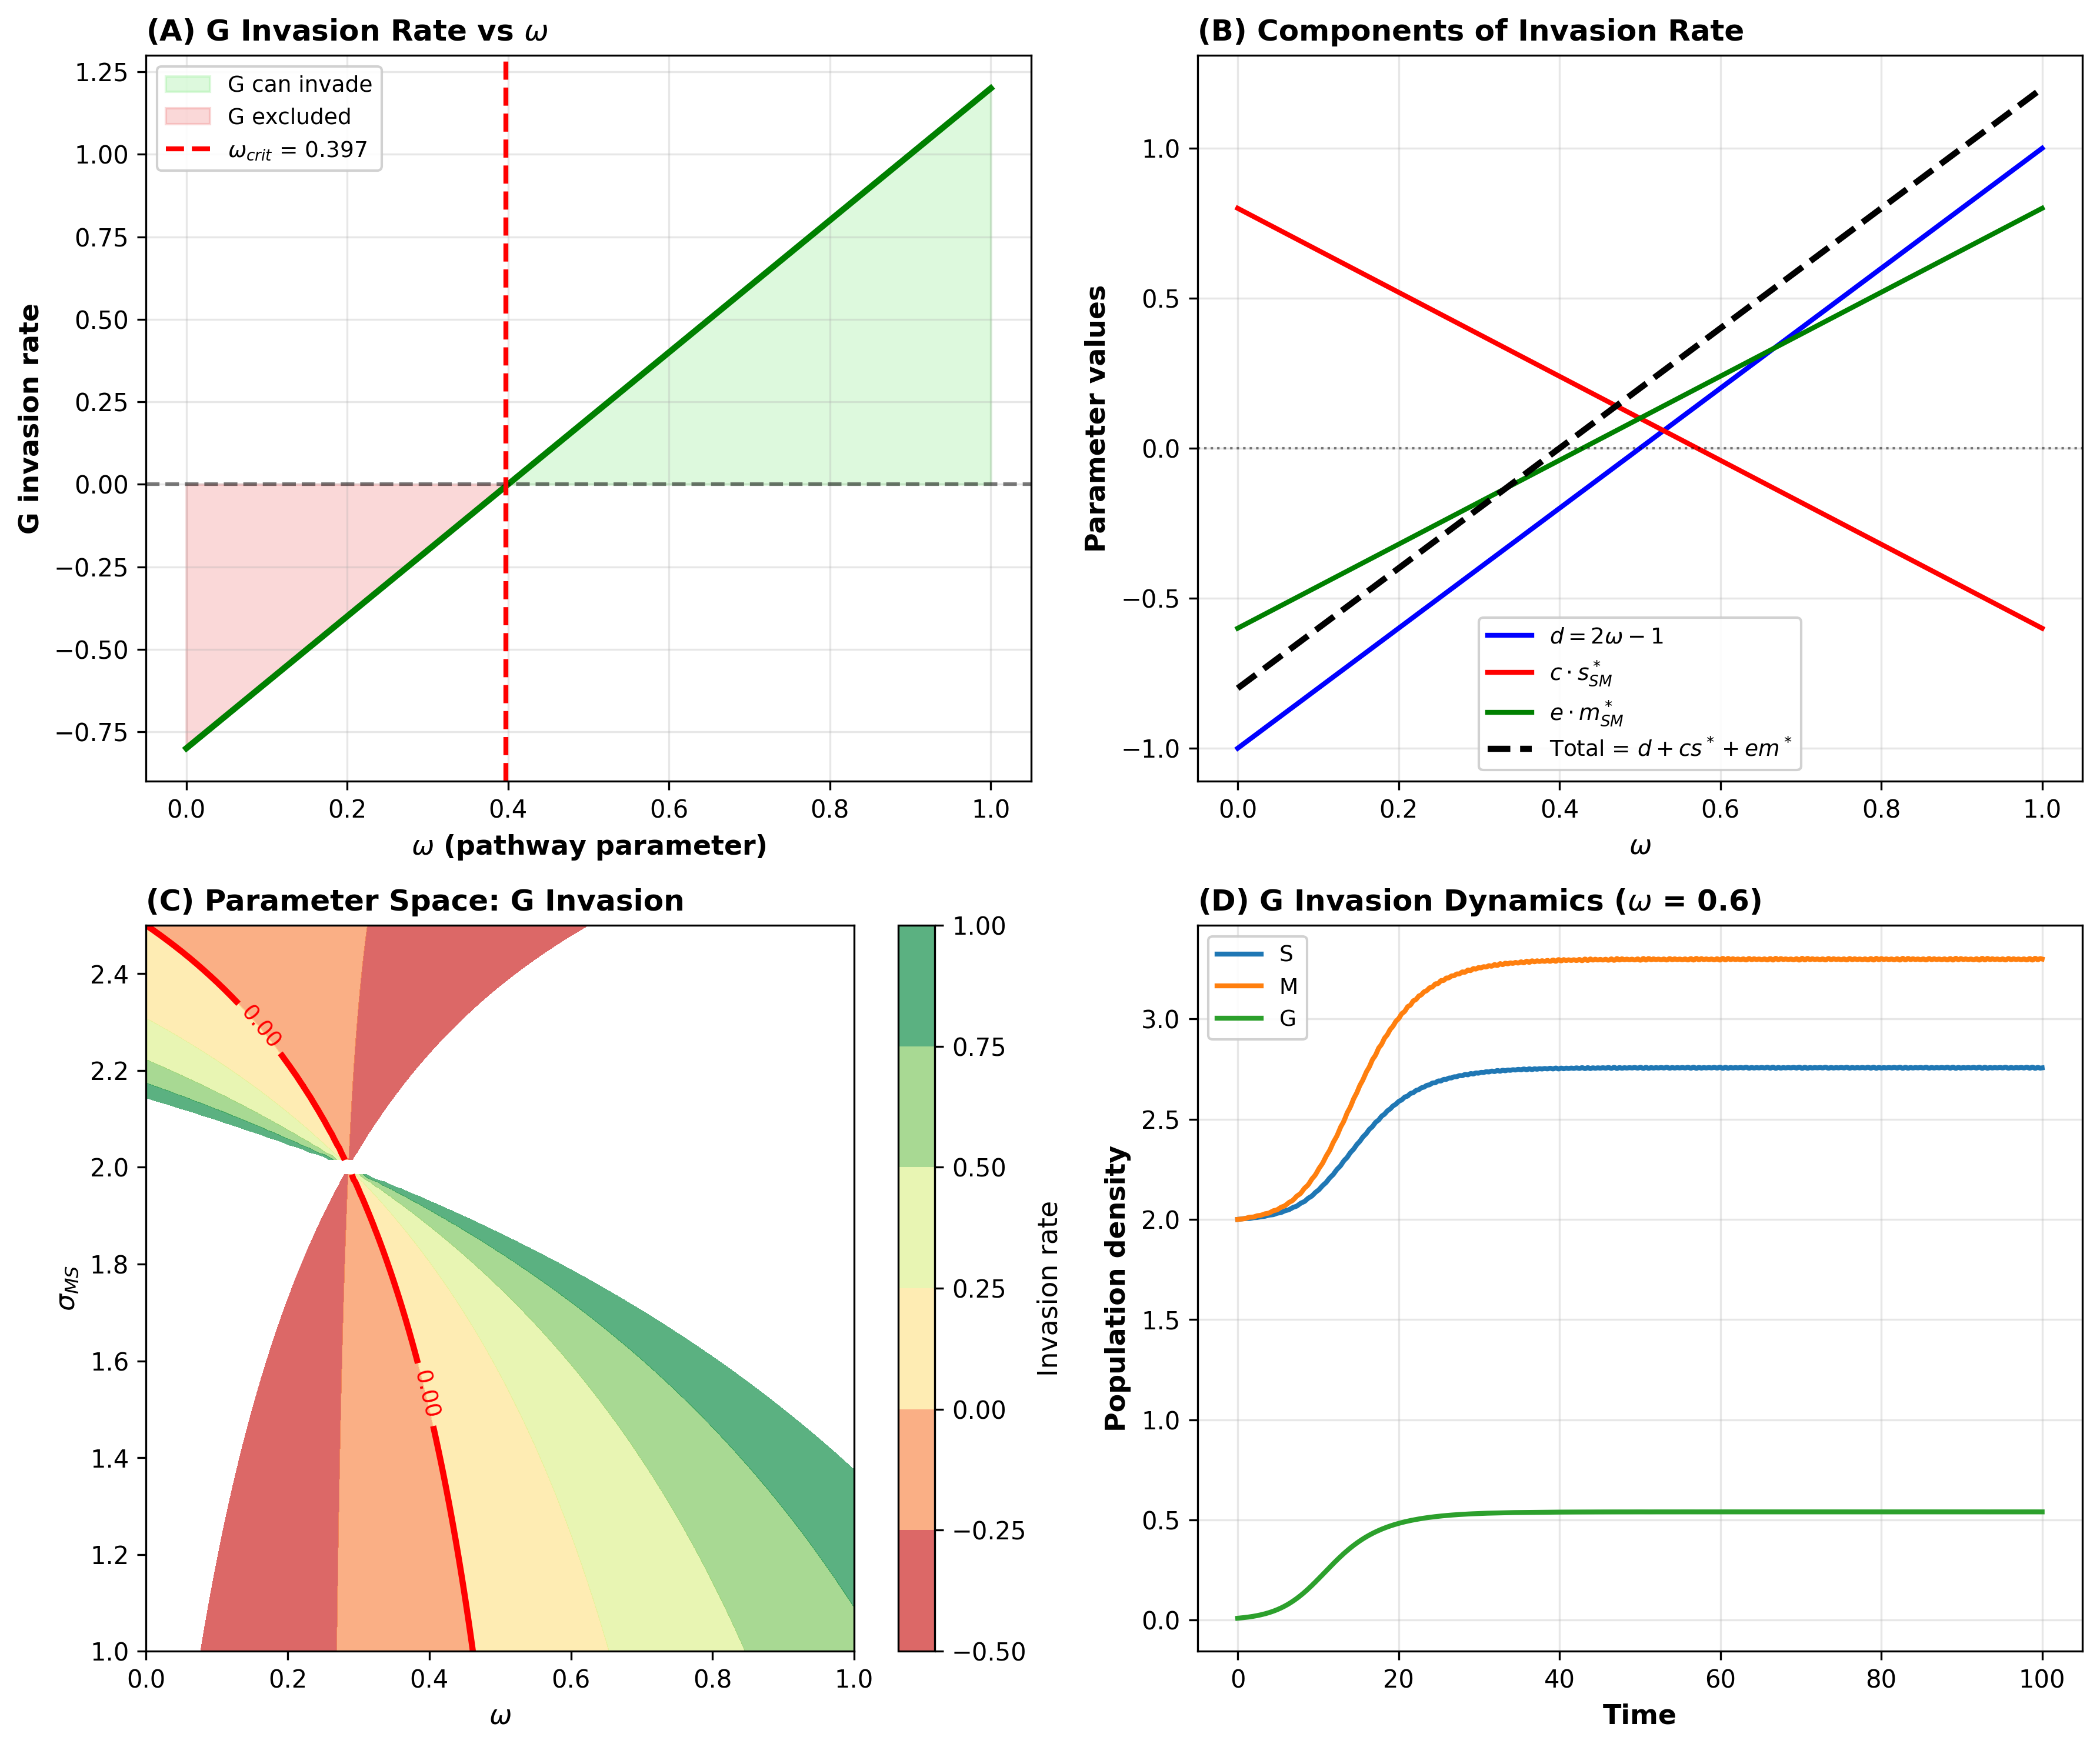
\includegraphics[width=\textwidth]{figures/Figure2_G_invasion.png}
\caption{\textbf{Generalist invasion of S-M consortia.} (A) G's invasion rate $\lambda_G$ as a function of $\omega$. Shaded regions indicate invasion (green) vs. exclusion (red). Red dashed line marks $\omega_{crit}$. (B) Components of invasion rate: basal term $d$, substrate-mediated term $c \cdot s^*_{SM}$, and metabolite-mediated term $e \cdot m^*_{SM}$. (C) Parameter space diagram in $(\omega, \sigma_{MS})$ plane. Contours show invasion rate; thick red line is the bifurcation boundary ($\lambda_G = 0$). (D) Time series demonstrating successful G invasion from small initial density when $\omega > \omega_{crit}$.}
\label{fig:invasion}
\end{figure}

\subsubsection{2.3 Bifurcation Analysis}

As $\omega$ increases from 0 to 1, the system undergoes a \textit{transcritical bifurcation}:

\textbf{Bifurcation Sequence:}

\begin{enumerate}
\item \textbf{$\omega < \omega_{crit1}$}: S-M coexistence is stable, G cannot invade. The system remains in $E_{SM}$ with $g = 0$.

\item \textbf{$\omega = \omega_{crit1}$}: \textit{First transcritical bifurcation.} The invasion rate $\lambda_G = 0$. $E_{SM}$ loses stability along the $g$-direction. An interior equilibrium $E^*$ emerges from the boundary.

\item \textbf{$\omega_{crit1} < \omega < \omega_{crit2}$}: \textit{Three-species coexistence window.} All three species coexist at a stable interior equilibrium. G has successfully invaded and established.

\item \textbf{$\omega = \omega_{crit2}$}: \textit{Second transcritical bifurcation.} M's density $m^* \to 0$. The interior equilibrium $E^*$ merges with the S-G boundary equilibrium $E_{SG}$.

\item \textbf{$\omega > \omega_{crit2}$}: S-G coexistence. M is excluded as G's substrate specialization makes it a superior competitor for resources.
\end{enumerate}

\textbf{Bifurcation Diagram:} Figure \ref{fig:bifurcation} shows equilibrium population densities vs. $\omega$:

\begin{itemize}
\item \textbf{S population (Panel A)}: Exhibits smooth transition from $s^*_{SM}$ to $s^*$ to $s^*_{SG}$.
\item \textbf{M population (Panel B)}: Non-zero only in $[\omega_{crit1}, \omega_{crit2}]$, decreasing as $\omega$ increases (G competes more for substrate).
\item \textbf{G population (Panel C)}: Jumps from 0 to positive at $\omega_{crit1}$ (transcritical bifurcation signature), increases with $\omega$.
\item \textbf{Combined view (Panel D)}: Golden shaded region marks three-species coexistence window. Red dashed lines indicate bifurcation points.
\end{itemize}

\begin{figure}[H]
\centering
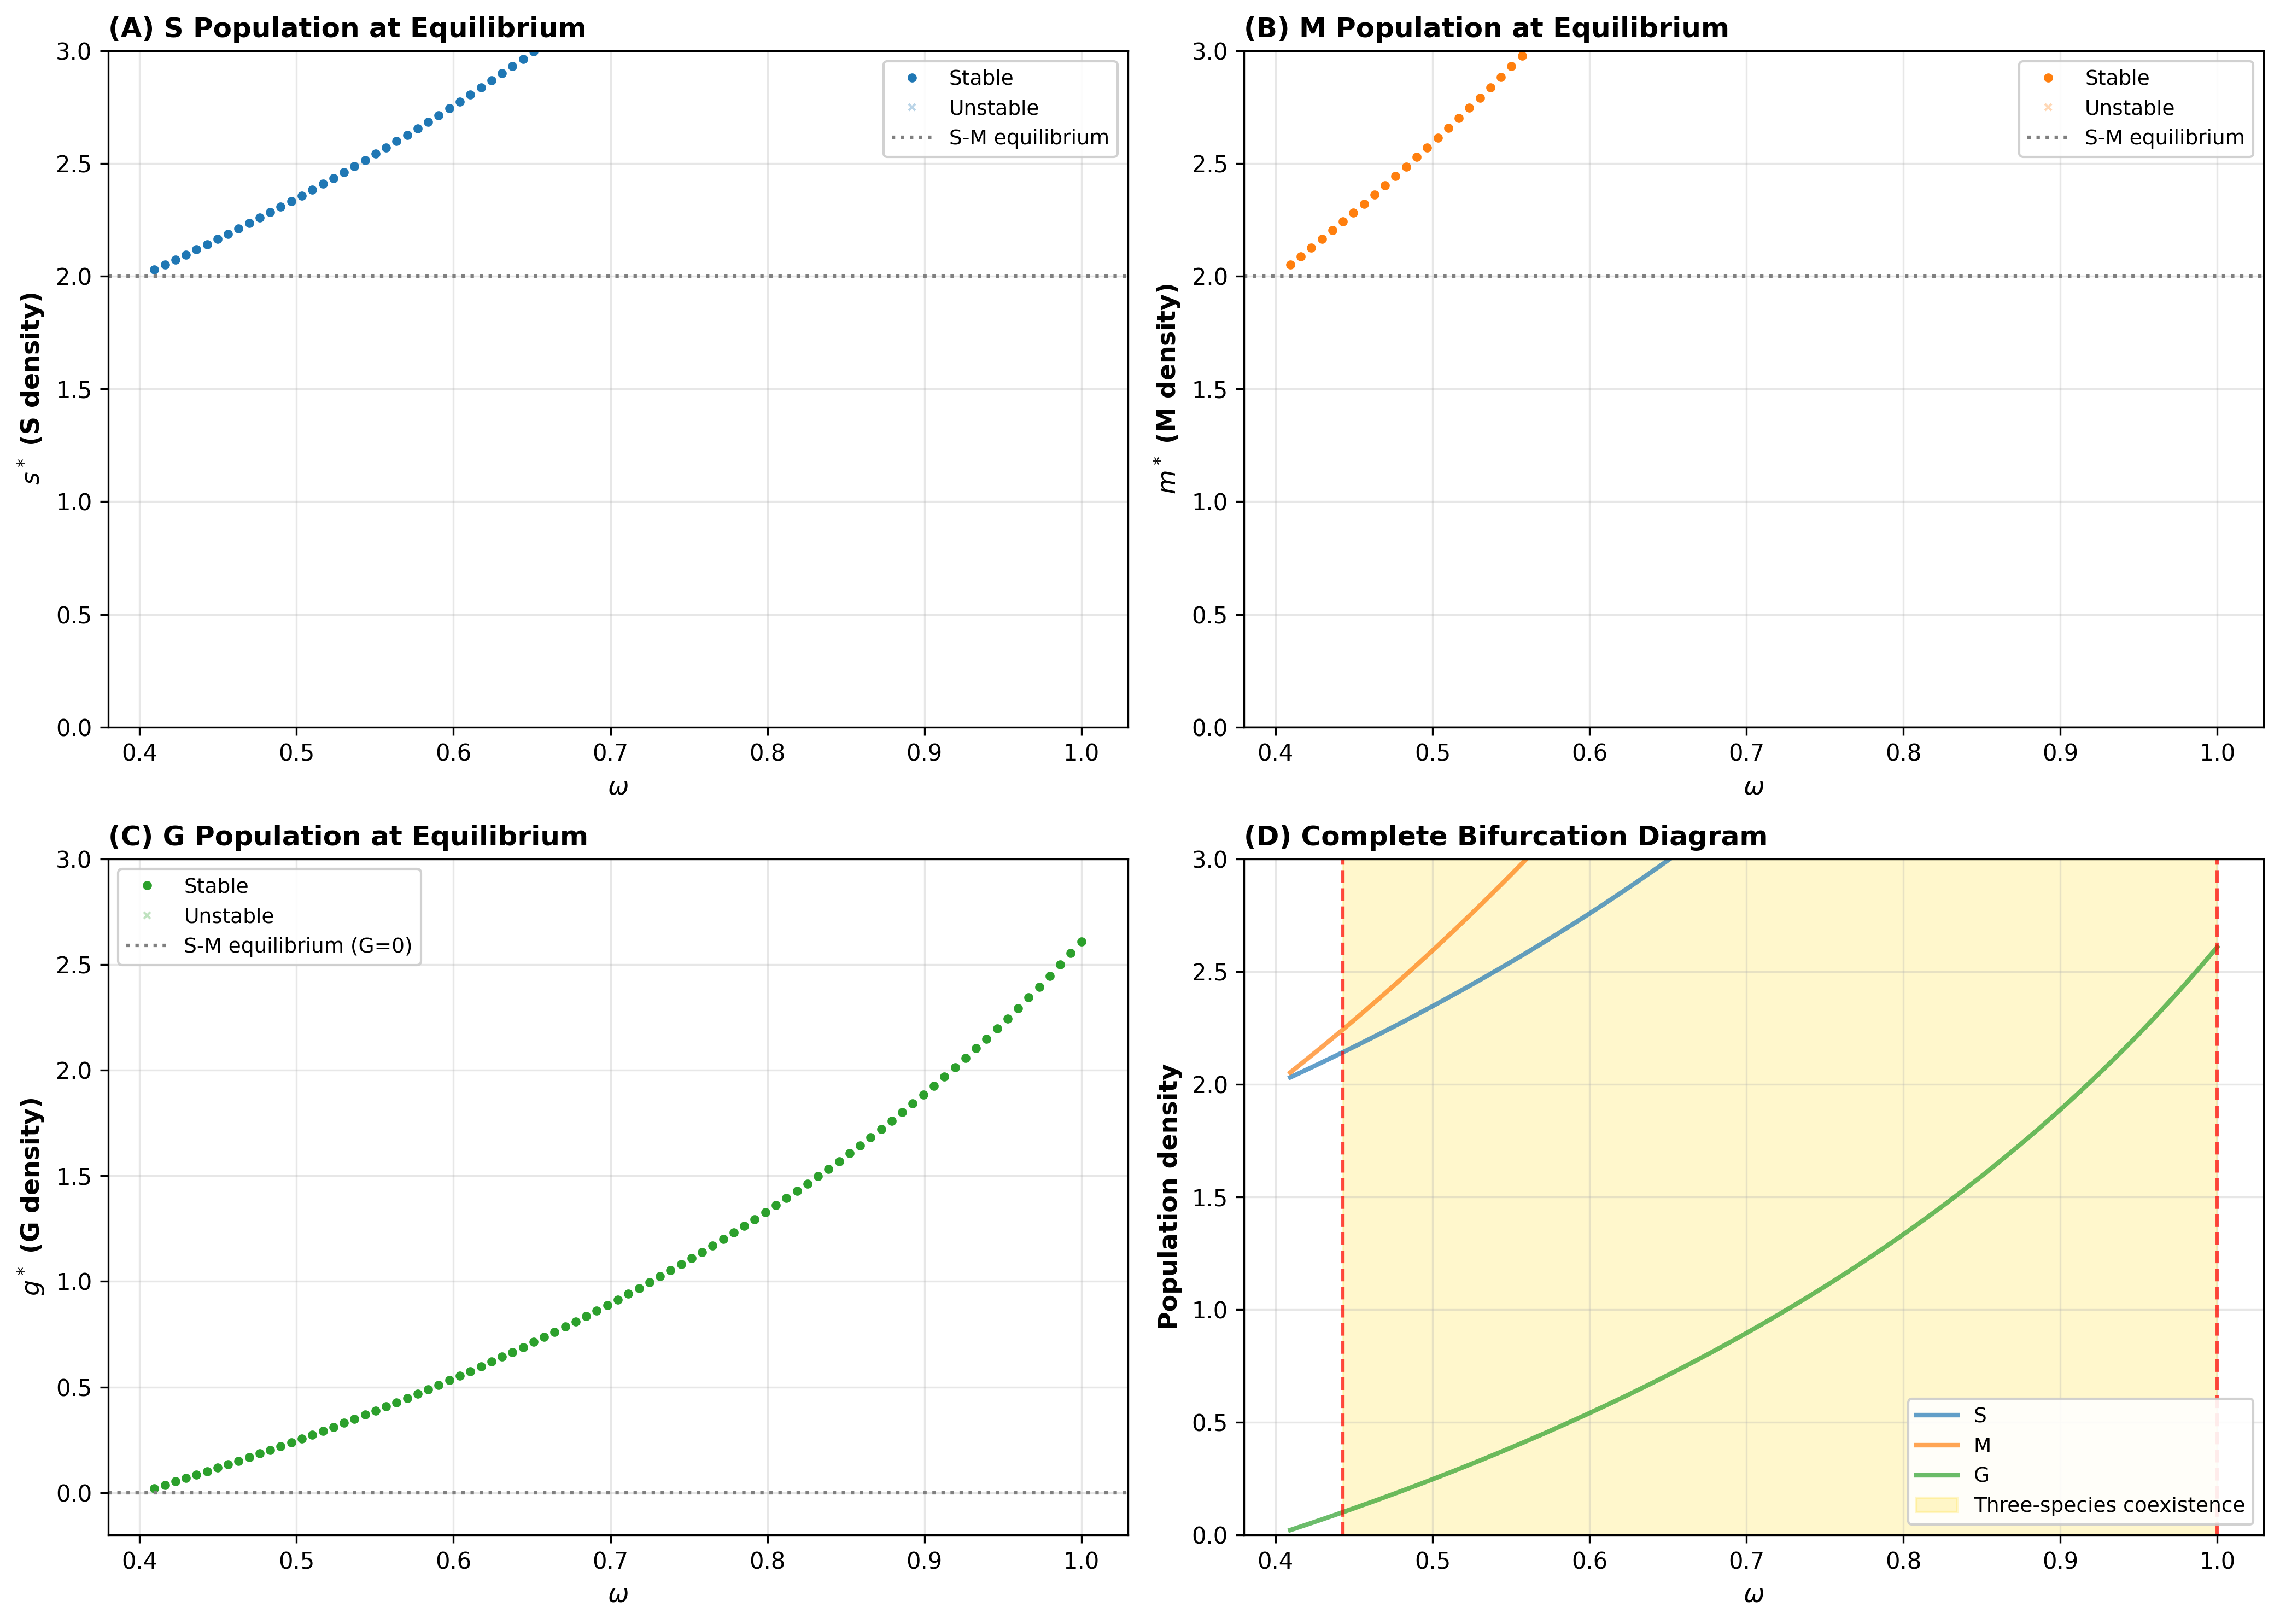
\includegraphics[width=\textwidth]{figures/Figure3_bifurcation_diagram.png}
\caption{\textbf{Complete bifurcation diagram with $\omega$ as bifurcation parameter.} Equilibrium population densities plotted against generalist pathway parameter $\omega$. Circles: stable equilibria; crosses: unstable. (A) S density shows smooth variation across bifurcations. Gray dotted line: S-M equilibrium level. (B) M density exists only in intermediate $\omega$ range, vanishing at $\omega_{crit2}$. (C) G density exhibits transcritical jump at $\omega_{crit1}$ where it invades from zero. (D) All species together. Golden region: three-species coexistence window bounded by transcritical bifurcations (red dashed lines). Parameters: $\sigma_{SM} = 0.5$, $\sigma_{MS} = 1.5$, other interaction parameters as specified in Methods.}
\label{fig:bifurcation}
\end{figure}

\textbf{Stability Analysis:} At the interior equilibrium $E^* = (s^*, m^*, g^*)$, the Jacobian is:

\begin{equation}
J = \begin{pmatrix}
-r_S s^* & r_S s^* \sigma_{SM} & r_S s^* a\\
r_M m^* \sigma_{MS} & -r_M m^* & r_M m^* b\\
r_G g^* c & r_G g^* e & -r_G g^*
\end{pmatrix}
\end{equation}

The trace is always negative (sum of diagonal elements):
\begin{equation}
\text{Tr}(J) = -(r_S s^* + r_M m^* + r_G g^*) < 0
\end{equation}

Stability requires all eigenvalues to have negative real parts. The determinant and Routh-Hurwitz criteria provide additional constraints:

\begin{equation}
\det(J) = -r_S r_M r_G s^* m^* g^* \left[1 - \sigma_{SM}\cdot\sigma_{MS} + \text{(G-dependent terms)}\right]
\end{equation}

Within the coexistence window, these criteria are satisfied, confirming stable three-species equilibrium.

\section{Discussion}

\subsection{Main Findings}

We have presented a complete analytical characterization of a three-species cross-feeding model with substrate specialists, metabolite specialists, and metabolically flexible generalists. Our key findings are:

\textbf{(1) Niche partitioning through metabolic flexibility:} The generalist can coexist with both specialists only when its metabolic strategy ($\omega$) occupies an intermediate range. Too metabolite-specialized, it competes with M; too substrate-specialized, it competes with S. This represents a form of \textit{metabolic niche differentiation}.

\textbf{(2) Transcritical bifurcation mechanism:} The transition from S-M to three-species community occurs via a transcritical bifurcation where equilibria exchange stability. This is distinct from saddle-node bifurcations (where equilibria disappear) and provides a smooth pathway for community assembly.

\textbf{(3) Critical invasion threshold:} We derived an explicit analytical formula for $\omega_{crit}$, the critical metabolic strategy enabling G invasion. This threshold depends on the S-M equilibrium structure, demonstrating how pairwise interactions constrain higher-order assembly.

\textbf{(4) Parameter-space structure:} The coexistence region forms a bounded window in $\omega$, flanked by competitive exclusion regimes. Width of this window depends on interaction strengths ($\sigma$, $\alpha$ parameters), providing design principles for synthetic consortia.

\subsection{Comparison with Previous Work}

Our work extends classic two-species mutualism models \cite{may1973stability,holland2002consumer} to include metabolically flexible third species. While obligate mutualisms (S-M type) have been studied extensively \cite{bronstein2015mutualism}, the role of generalists in stabilizing or destabilizing such partnerships is less understood.

Recent experimental work on cross-feeding yeast \cite{shou2007synthetic,goldschmidt2017successive} and bacteria \cite{mee2014syntrophic,harcombe2014metabolic} has demonstrated metabolic division of labor, but theoretical frameworks often focus on pairwise interactions. Our model provides a bridge to more complex communities by explicitly incorporating metabolic flexibility.

The transcritical bifurcation structure we identify echoes findings in other ecological contexts, such as adaptive dynamics \cite{geritz1998evolutionarily} and evolutionary branching \cite{doebeli2003speciation}, where strategies evolve to occupy intermediate niches.

\subsection{Biological Implications}

\textbf{Metabolic trade-offs and coexistence:} Our model predicts that generalists must balance pathway usage to coexist with specialists. This aligns with the jack-of-all-trades-master-of-none principle: generalists sacrifice efficiency for niche breadth.

\textbf{Community assembly rules:} The sequential invasion process (first M invades S, then G invades S-M) suggests historical contingency in community assembly. Order of arrival and metabolic strategies jointly determine final composition.

\textbf{Synthetic consortium design:} For engineering stable three-species systems, our results suggest:
\begin{itemize}
\item Choose $\sigma_{MS}$ sufficiently large (> 1) to ensure M viability.
\item Tune $\sigma_{MS}\cdot\sigma_{SM} < 1$ to prevent runaway mutualism.
\item Engineer G with intermediate $\omega \in (\omega_{crit1}, \omega_{crit2})$ for stable coexistence.
\item Avoid $\omega$ extremes to prevent competitive exclusion.
\end{itemize}

\subsection{Limitations and Extensions}

Our model makes several simplifying assumptions:

\textbf{Well-mixed environment:} Spatial structure can stabilize coexistence through local interactions \cite{momeni2013strong,dal2014resource}. Extending to spatial models (e.g., cellular automata, reaction-diffusion) could reveal additional mechanisms.

\textbf{Constant parameters:} In reality, $\omega$ may evolve or respond plastically to environment. Incorporating adaptive dynamics would allow studying evolutionary stability of metabolic strategies.

\textbf{Two resources:} Our model considers substrate and metabolite. Natural communities involve multiple resource types and more complex food webs. Extensions to $n$-species, $m$-resource systems could capture richer dynamics.

\textbf{Deterministic framework:} Stochastic effects (demographic noise, environmental fluctuations) can qualitatively change outcomes, especially near bifurcations. Stochastic differential equation formulations would address this.

Despite these limitations, the model captures essential features of cross-feeding communities and provides quantitative, testable predictions.

\subsection{Experimental Predictions}

Our theory makes several predictions amenable to experimental testing:

\begin{enumerate}
\item \textbf{Critical $\omega$ threshold:} By engineering strains with tunable pathway expression (e.g., inducible promoters controlling substrate vs. metabolite utilization genes), one could map the predicted coexistence window.

\item \textbf{Bifurcation signatures:} Gradually increasing $\omega$ (e.g., via chemostat dilution rate or inducer concentration) should exhibit sudden appearance of G (at $\omega_{crit1}$) and disappearance of M (at $\omega_{crit2}$).

\item \textbf{Invasion dynamics:} Starting with stable S-M communities and introducing G at different $\omega$ values, invasion success should correlate with $\omega > \omega_{crit1}$.

\item \textbf{Parameter sensitivity:} Varying S-M mutualism strength ($\sigma_{MS}$) should shift $\omega_{crit}$ as predicted by our formula.
\end{enumerate}

Systems such as engineered \textit{E. coli} or yeast strains with well-characterized metabolic pathways \cite{wintermute2010dynamics,mee2014syntrophic} are ideal candidates for these tests.

\section{Conclusion}

We have developed a comprehensive analytical framework for understanding how metabolically flexible generalists integrate into cross-feeding communities. By identifying transcritical bifurcations as the assembly mechanism, deriving explicit invasion criteria, and mapping the parameter space, we provide both fundamental insights and practical guidelines. Our work underscores the importance of metabolic niche partitioning—not just resource partitioning—in microbial coexistence. As synthetic biology advances our ability to engineer metabolic strategies, theoretical frameworks like ours become essential for rational community design. Future work integrating spatial structure, evolutionary dynamics, and experimental validation will further bridge theory and application in microbial ecology.

\section*{Methods}

\subsection{Parameter Values}

Unless otherwise stated, we use the following baseline parameters:
\begin{itemize}
\item Growth rates: $r_S = 1.0$, $r_M = 0.8$, $r_G = 0.9$ (day$^{-1}$)
\item S-M interactions: $\sigma_{SM} = 0.5$, $\sigma_{MS} = 1.5$
\item S-G interactions: $\sigma_{SG} = 0.3$, $\sigma_{GS} = 0.4$, $\alpha_{SG} = 0.4$, $\alpha_{GS} = 0.3$
\item M-G interactions: $\sigma_{MG} = 0.3$, $\sigma_{GM} = 0.4$, $\alpha_{MG} = 0.4$, $\alpha_{GM} = 0.3$
\item Pathway parameter: $\omega \in [0, 1]$ (varied as bifurcation parameter)
\end{itemize}

These values are chosen to represent: (i) obligate M dependence ($\sigma_{MS} > 1$), (ii) stable S-M mutualism ($\sigma_{MS}\cdot\sigma_{SM} < 1$), and (iii) balanced cooperation/competition for G.

\subsection{Numerical Methods}

\textbf{ODE integration:} Time series were computed using SciPy's \texttt{solve\_ivp} with the RK45 method, relative tolerance $10^{-6}$, absolute tolerance $10^{-8}$.

\textbf{Equilibrium finding:} Interior equilibria were found by numerically solving the system $\mathbf{F}(\mathbf{N}^*) = 0$ using \texttt{fsolve} with multiple initial guesses.

\textbf{Stability analysis:} Eigenvalues of the Jacobian were computed using NumPy's \texttt{linalg.eigvals}. Equilibria with all $\text{Re}(\lambda_i) < 0$ were classified as stable.

\textbf{Bifurcation diagrams:} For each $\omega \in [0, 1]$ (200 points), we found equilibria, determined stability, and plotted results. Coexistence windows were identified where $g^* > 0.01$.

\textbf{Code availability:} All analysis code is available at [repository link].

\section*{Acknowledgments}

We thank [collaborators] for helpful discussions. This work was supported by [funding sources].

\begin{thebibliography}{99}

\bibitem{goldford2018emergent}
Goldford, J. E. et al. (2018). Emergent simplicity in microbial community assembly. \textit{Science}, 361(6401), 469--474.

\bibitem{pacheco2019costless}
Pacheco, A. R., Moel, M., \& Segrè, D. (2019). Costless metabolic secretions as drivers of interspecies interactions in microbial ecosystems. \textit{Nature Communications}, 10(1), 103.

\bibitem{ponomarova2017metabolic}
Ponomarova, O., \& Patil, K. R. (2015). Metabolic interactions in microbial communities: untangling the Gordian knot. \textit{Current Opinion in Microbiology}, 27, 37--44.

\bibitem{gore2009snowdrift}
Gore, J., Youk, H., \& Van Oudenaarden, A. (2009). Snowdrift game dynamics and facultative cheating in yeast. \textit{Nature}, 459(7244), 253--256.

\bibitem{harcombe2014metabolic}
Harcombe, W. R. et al. (2014). Metabolic resource allocation in individual microbes determines ecosystem interactions and spatial dynamics. \textit{Cell Reports}, 7(4), 1104--1115.

\bibitem{klitgord2010environments}
Klitgord, N., \& Segrè, D. (2010). Environments that induce synthetic microbial ecosystems. \textit{PLoS Computational Biology}, 6(11), e1001002.

\bibitem{zelezniak2015metabolic}
Zelezniak, A. et al. (2015). Metabolic dependencies drive species co-occurrence in diverse microbial communities. \textit{Proceedings of the National Academy of Sciences}, 112(20), 6449--6454.

\bibitem{momeni2011spatial}
Momeni, B., Brileya, K. A., Fields, M. W., \& Shou, W. (2013). Strong inter-population cooperation leads to partner intermixing in microbial communities. \textit{eLife}, 2, e00230.

\bibitem{muller2014venn}
Müller, M. J., Neugeboren, B. I., Nelson, D. R., \& Murray, A. W. (2014). Genetic drift opposes mutualism during spatial population expansion. \textit{Proceedings of the National Academy of Sciences}, 111(3), 1037--1042.

\bibitem{schink2002syntrophic}
Schink, B. (2002). Synergistic interactions in the microbial world. \textit{Antonie van Leeuwenhoek}, 81(1-4), 257--261.

\bibitem{may1973stability}
May, R. M. (1973). \textit{Stability and Complexity in Model Ecosystems}. Princeton University Press.

\bibitem{holland2002consumer}
Holland, J. N., \& DeAngelis, D. L. (2010). A consumer--resource approach to the density-dependent population dynamics of mutualism. \textit{Ecology}, 91(5), 1286--1295.

\bibitem{bronstein2015mutualism}
Bronstein, J. L. (Ed.). (2015). \textit{Mutualism}. Oxford University Press.

\bibitem{shou2007synthetic}
Shou, W., Ram, S., \& Vilar, J. M. (2007). Synthetic cooperation in engineered yeast populations. \textit{Proceedings of the National Academy of Sciences}, 104(6), 1877--1882.

\bibitem{goldschmidt2017successive}
Goldschmidt, F., Regoes, R. R., \& Johnson, D. R. (2017). Successive range expansion promotes diversity and accelerates evolution in spatially structured microbial populations. \textit{The ISME Journal}, 11(9), 2112--2123.

\bibitem{mee2014syntrophic}
Mee, M. T., Collins, J. J., Church, G. M., \& Wang, H. H. (2014). Syntrophic exchange in synthetic microbial communities. \textit{Proceedings of the National Academy of Sciences}, 111(20), E2149--E2156.

\bibitem{geritz1998evolutionarily}
Geritz, S. A., Kisdi, É., Meszéna, G., \& Metz, J. A. (1998). Evolutionarily singular strategies and the adaptive growth and branching of the evolutionary tree. \textit{Evolutionary Ecology}, 12(1), 35--57.

\bibitem{doebeli2003speciation}
Doebeli, M., \& Dieckmann, U. (2003). Speciation along environmental gradients. \textit{Nature}, 421(6920), 259--264.

\bibitem{momeni2013strong}
Momeni, B., Waite, A. J., \& Shou, W. (2013). Spatial self-organization favors heterotypic cooperation over cheating. \textit{eLife}, 2, e00960.

\bibitem{dal2014resource}
Dal Bello, M., Lee, H., Goyal, A., \& Gore, J. (2021). Resource–diversity relationships in bacterial communities reflect the network structure of microbial metabolism. \textit{Nature Ecology \& Evolution}, 5(10), 1424--1434.

\bibitem{wintermute2010dynamics}
Wintermute, E. H., \& Silver, P. A. (2010). Dynamics in the mixed microbial concourse. \textit{Genes \& Development}, 24(23), 2603--2614.

\end{thebibliography}

\end{document}
